\documentclass{article}

% ------------------------------------ %
%             Document Info            %
% ------------------------------------ %

\usepackage{../../../LaTeX-Preamables/Assign}

\begin{document}
\newcommand{\documentcourse}{ENGG1300}
\newcommand{\documentnumber}{3}

% ------------------------------------ %
%                Header                %
% ------------------------------------ %

\begin{minipage}{0.07\textwidth}
    
\includegraphics[width=\linewidth]{../../../LaTeX-Preamables/LaTeX-Templates/HKULOGO256.png}
\end{minipage}
\hspace{0.02\textwidth}
\begin{minipage}{0.55\textwidth}
    \documentcourse

    Assignment \documentnumber

    SID: 3036268218
\end{minipage}
\begin{minipage}{0.35\textwidth}
    \begin{flushright}
        Jax

        \jobname.pdf

        \today
    \end{flushright}
\end{minipage}

\vspace{0.5cm}

\hrule

% ------------------------------------ %
%                Content               %
% ------------------------------------ %
\centering
\section*{Question 1}
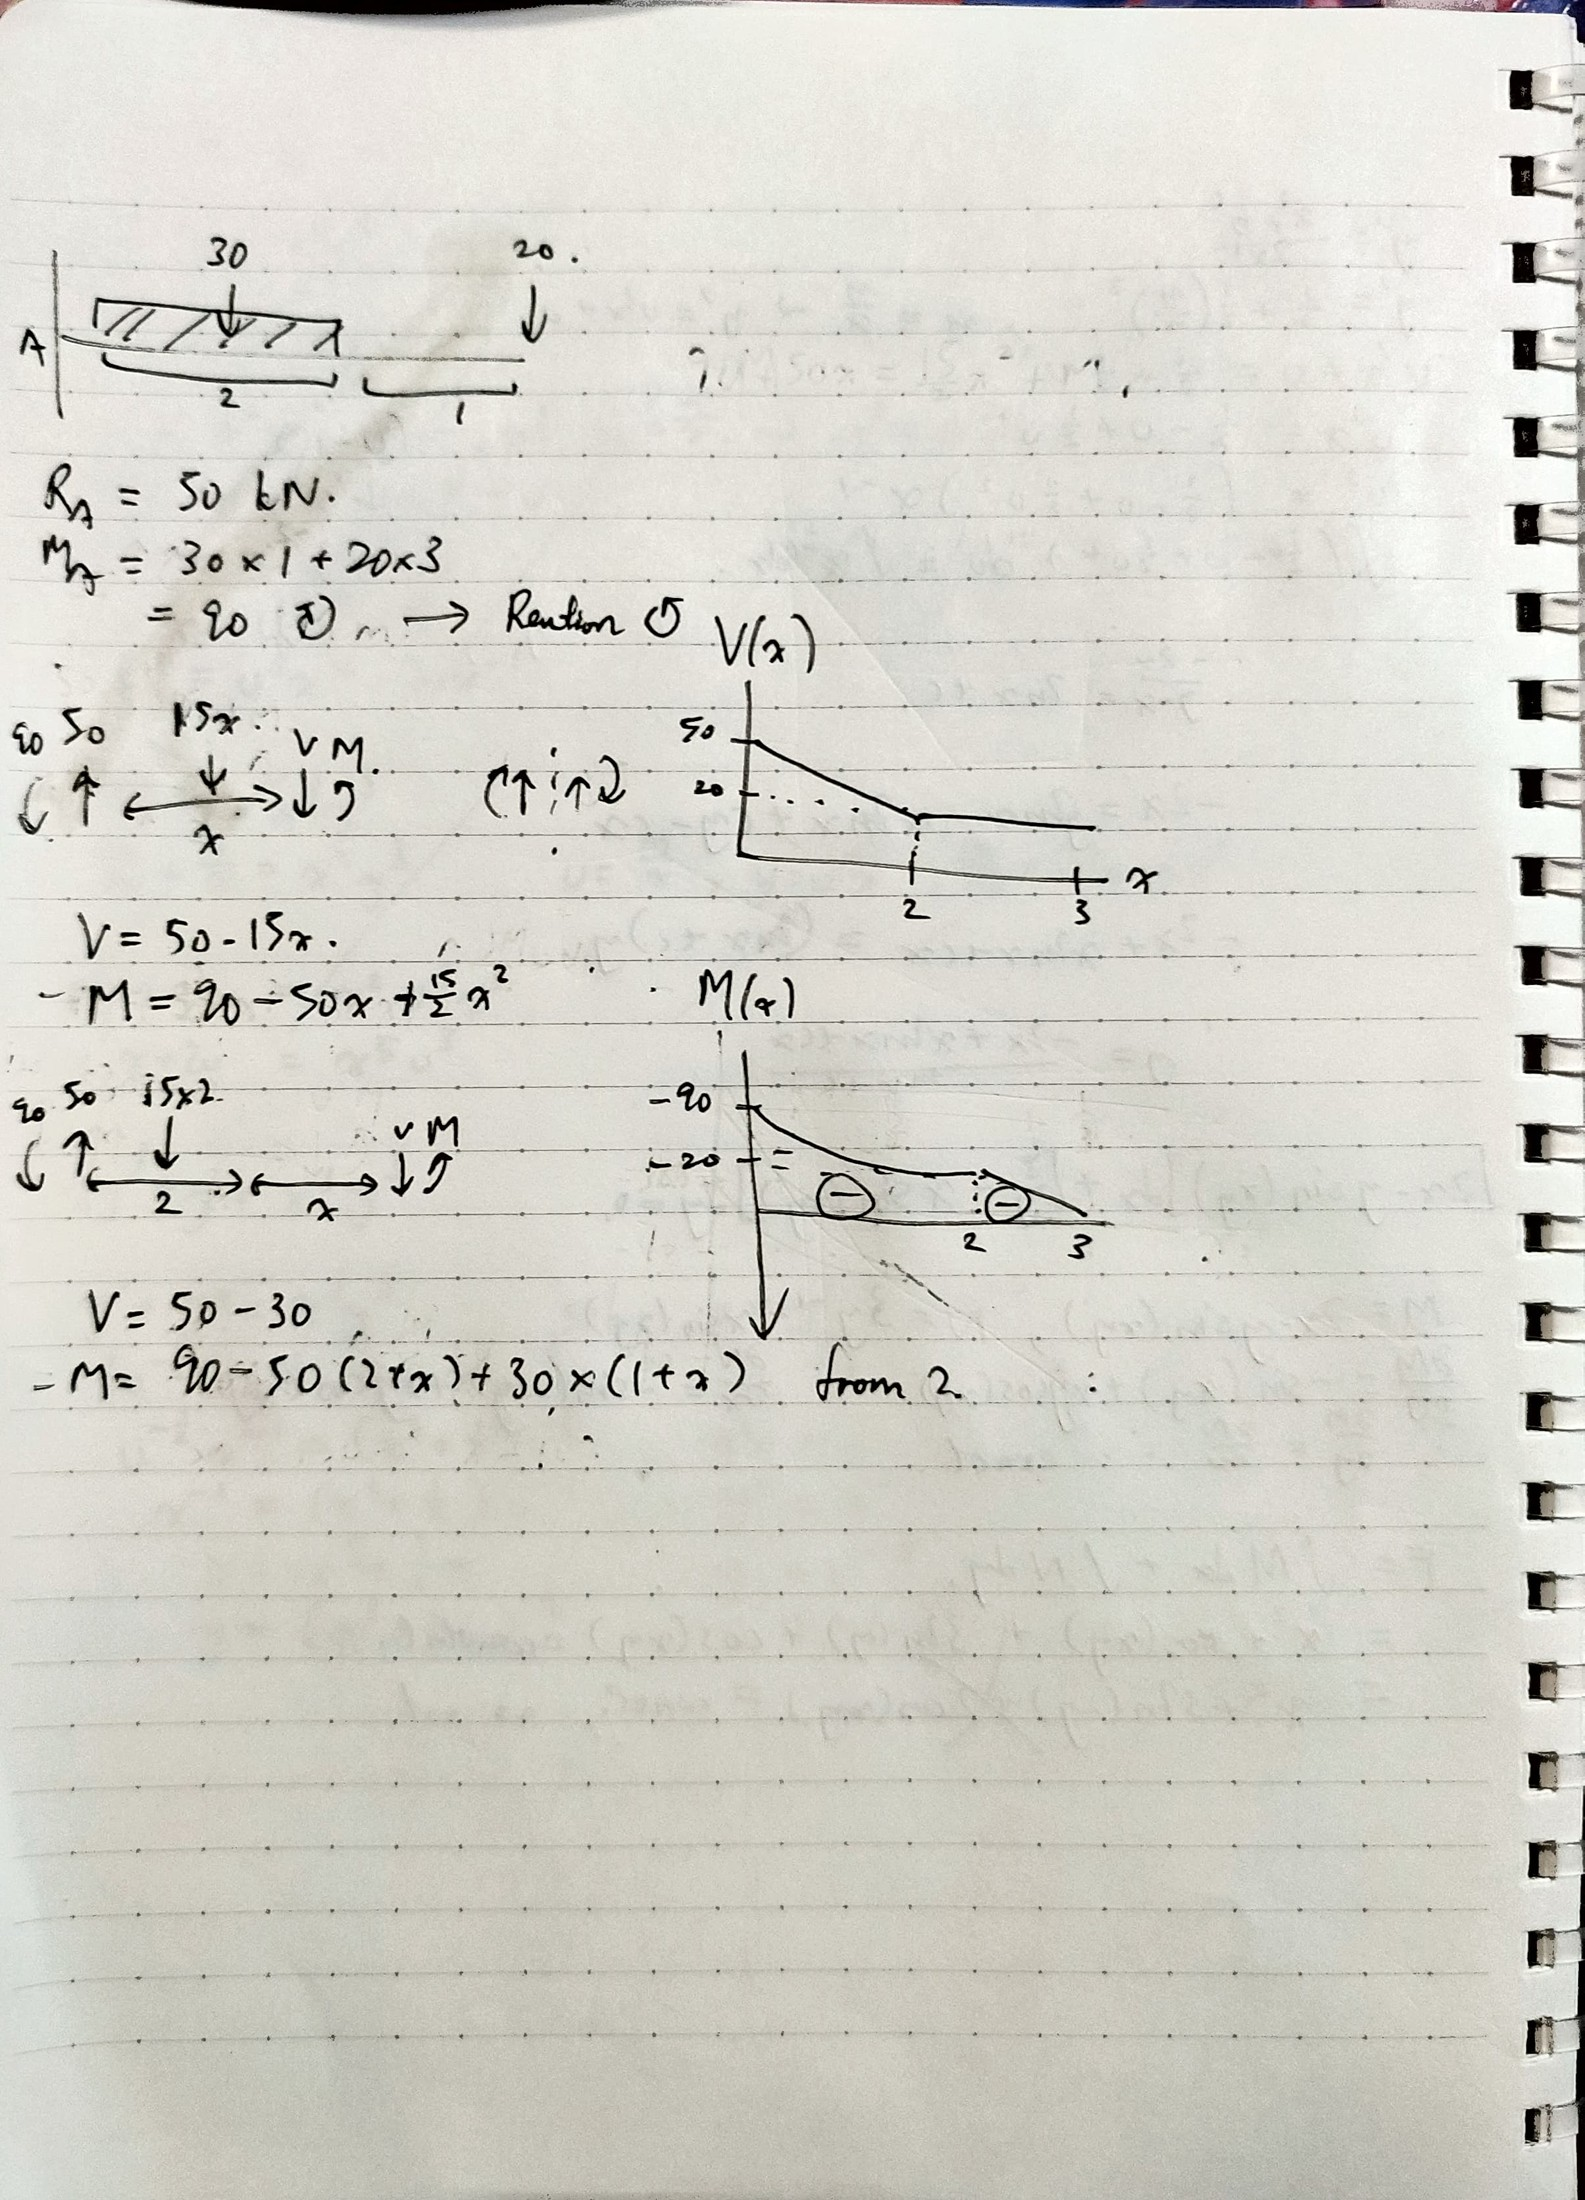
\includegraphics[width=0.7\textwidth]{img/A3Q1.jpg}
\section*{Question 2}
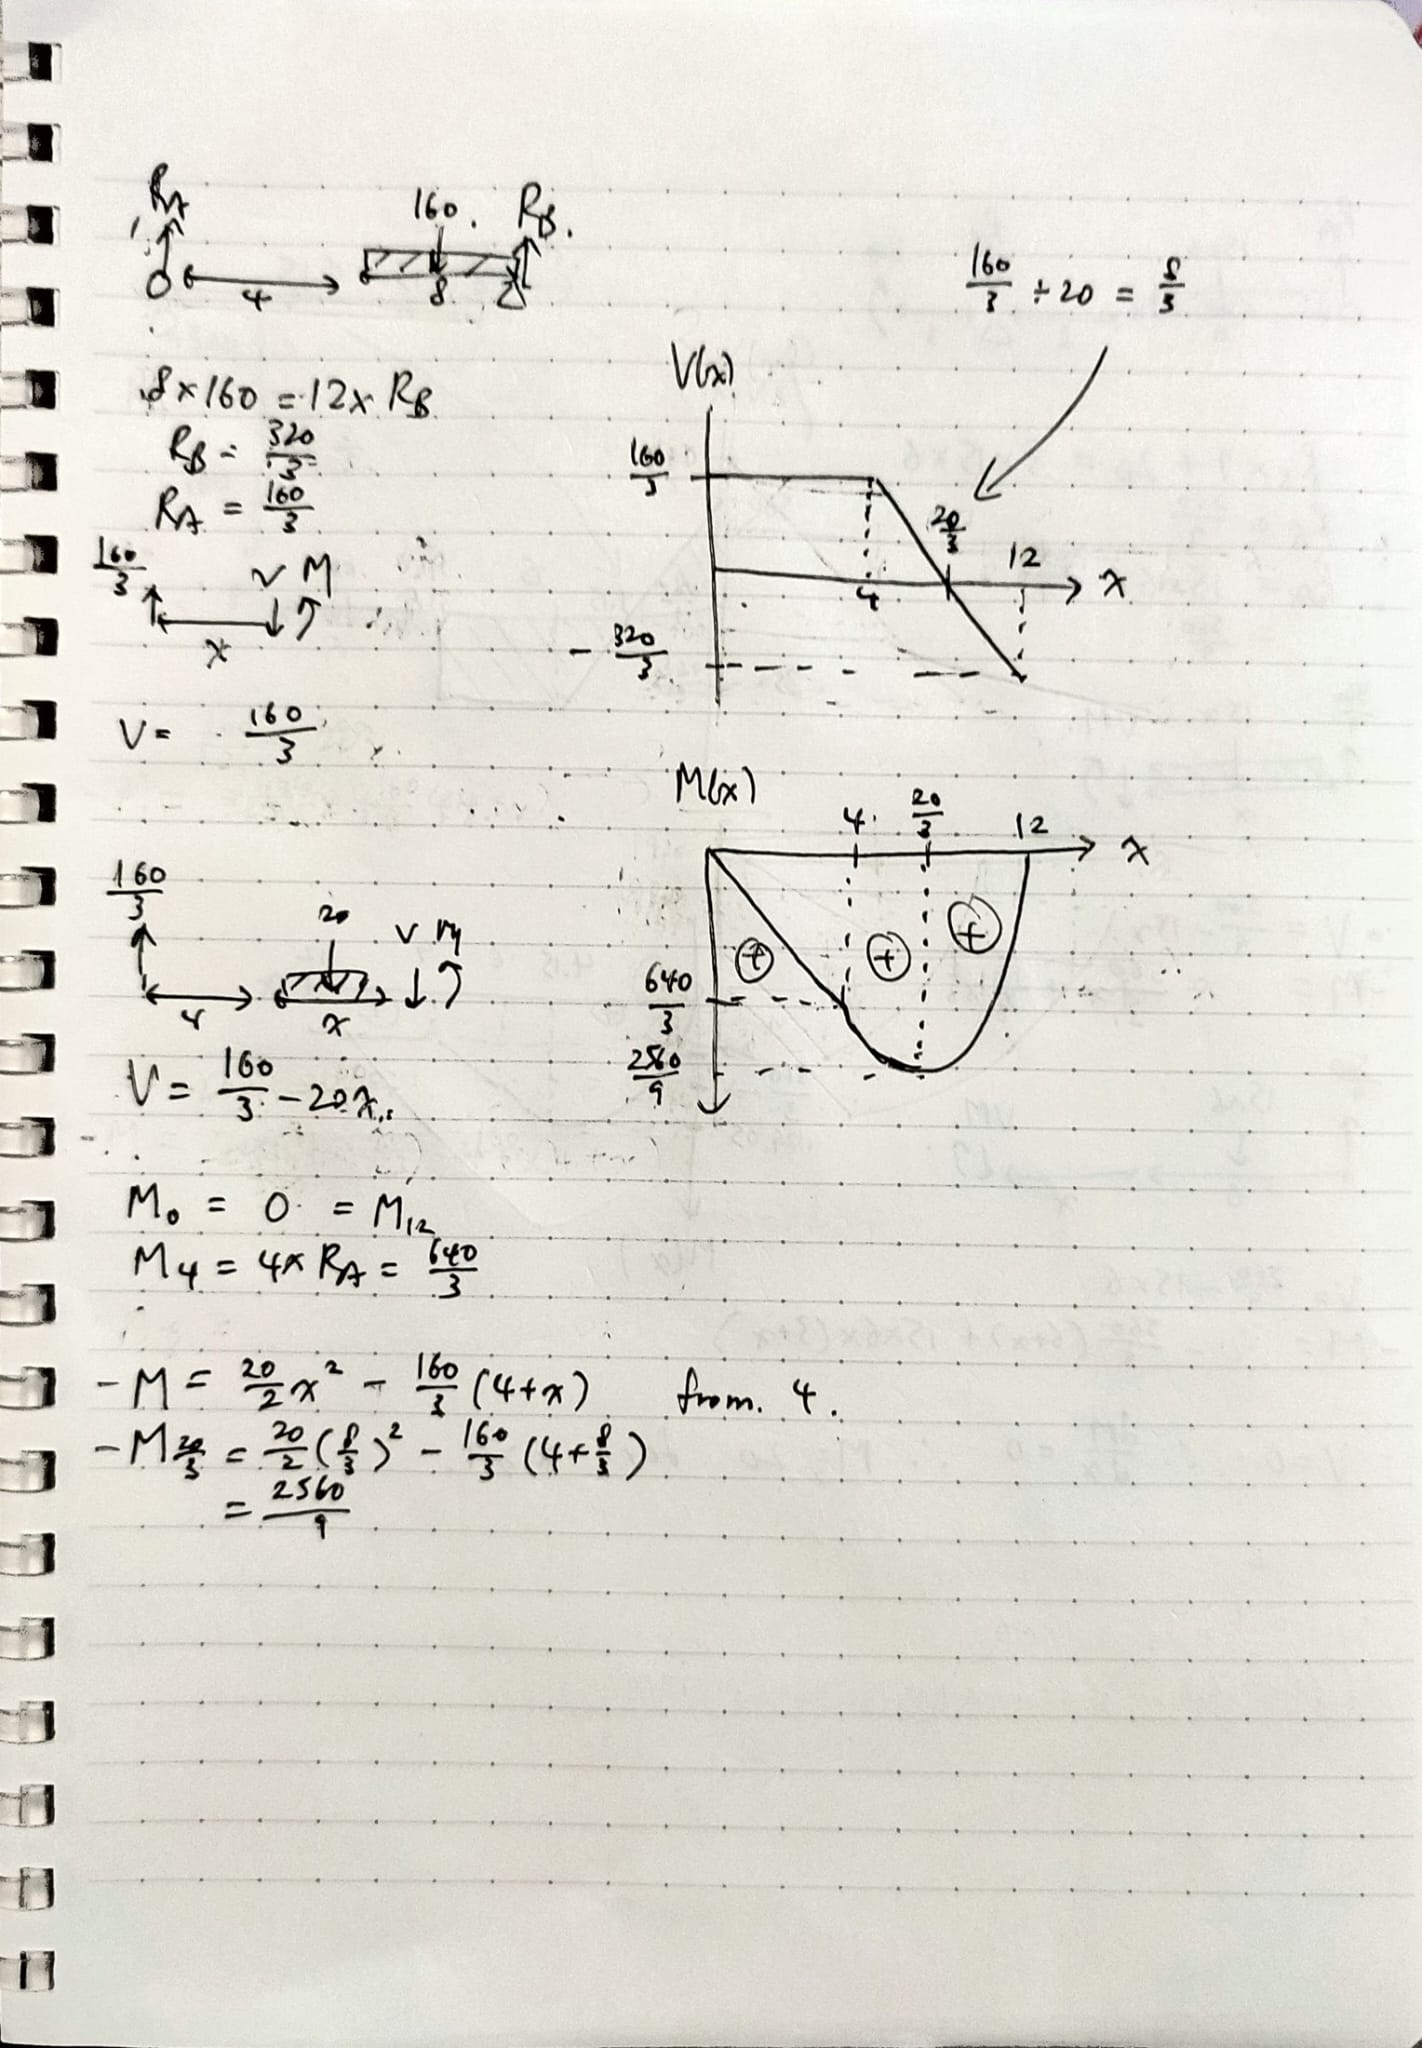
\includegraphics[width=0.7\textwidth]{img/A3Q2.jpeg}
\section*{Question 3}
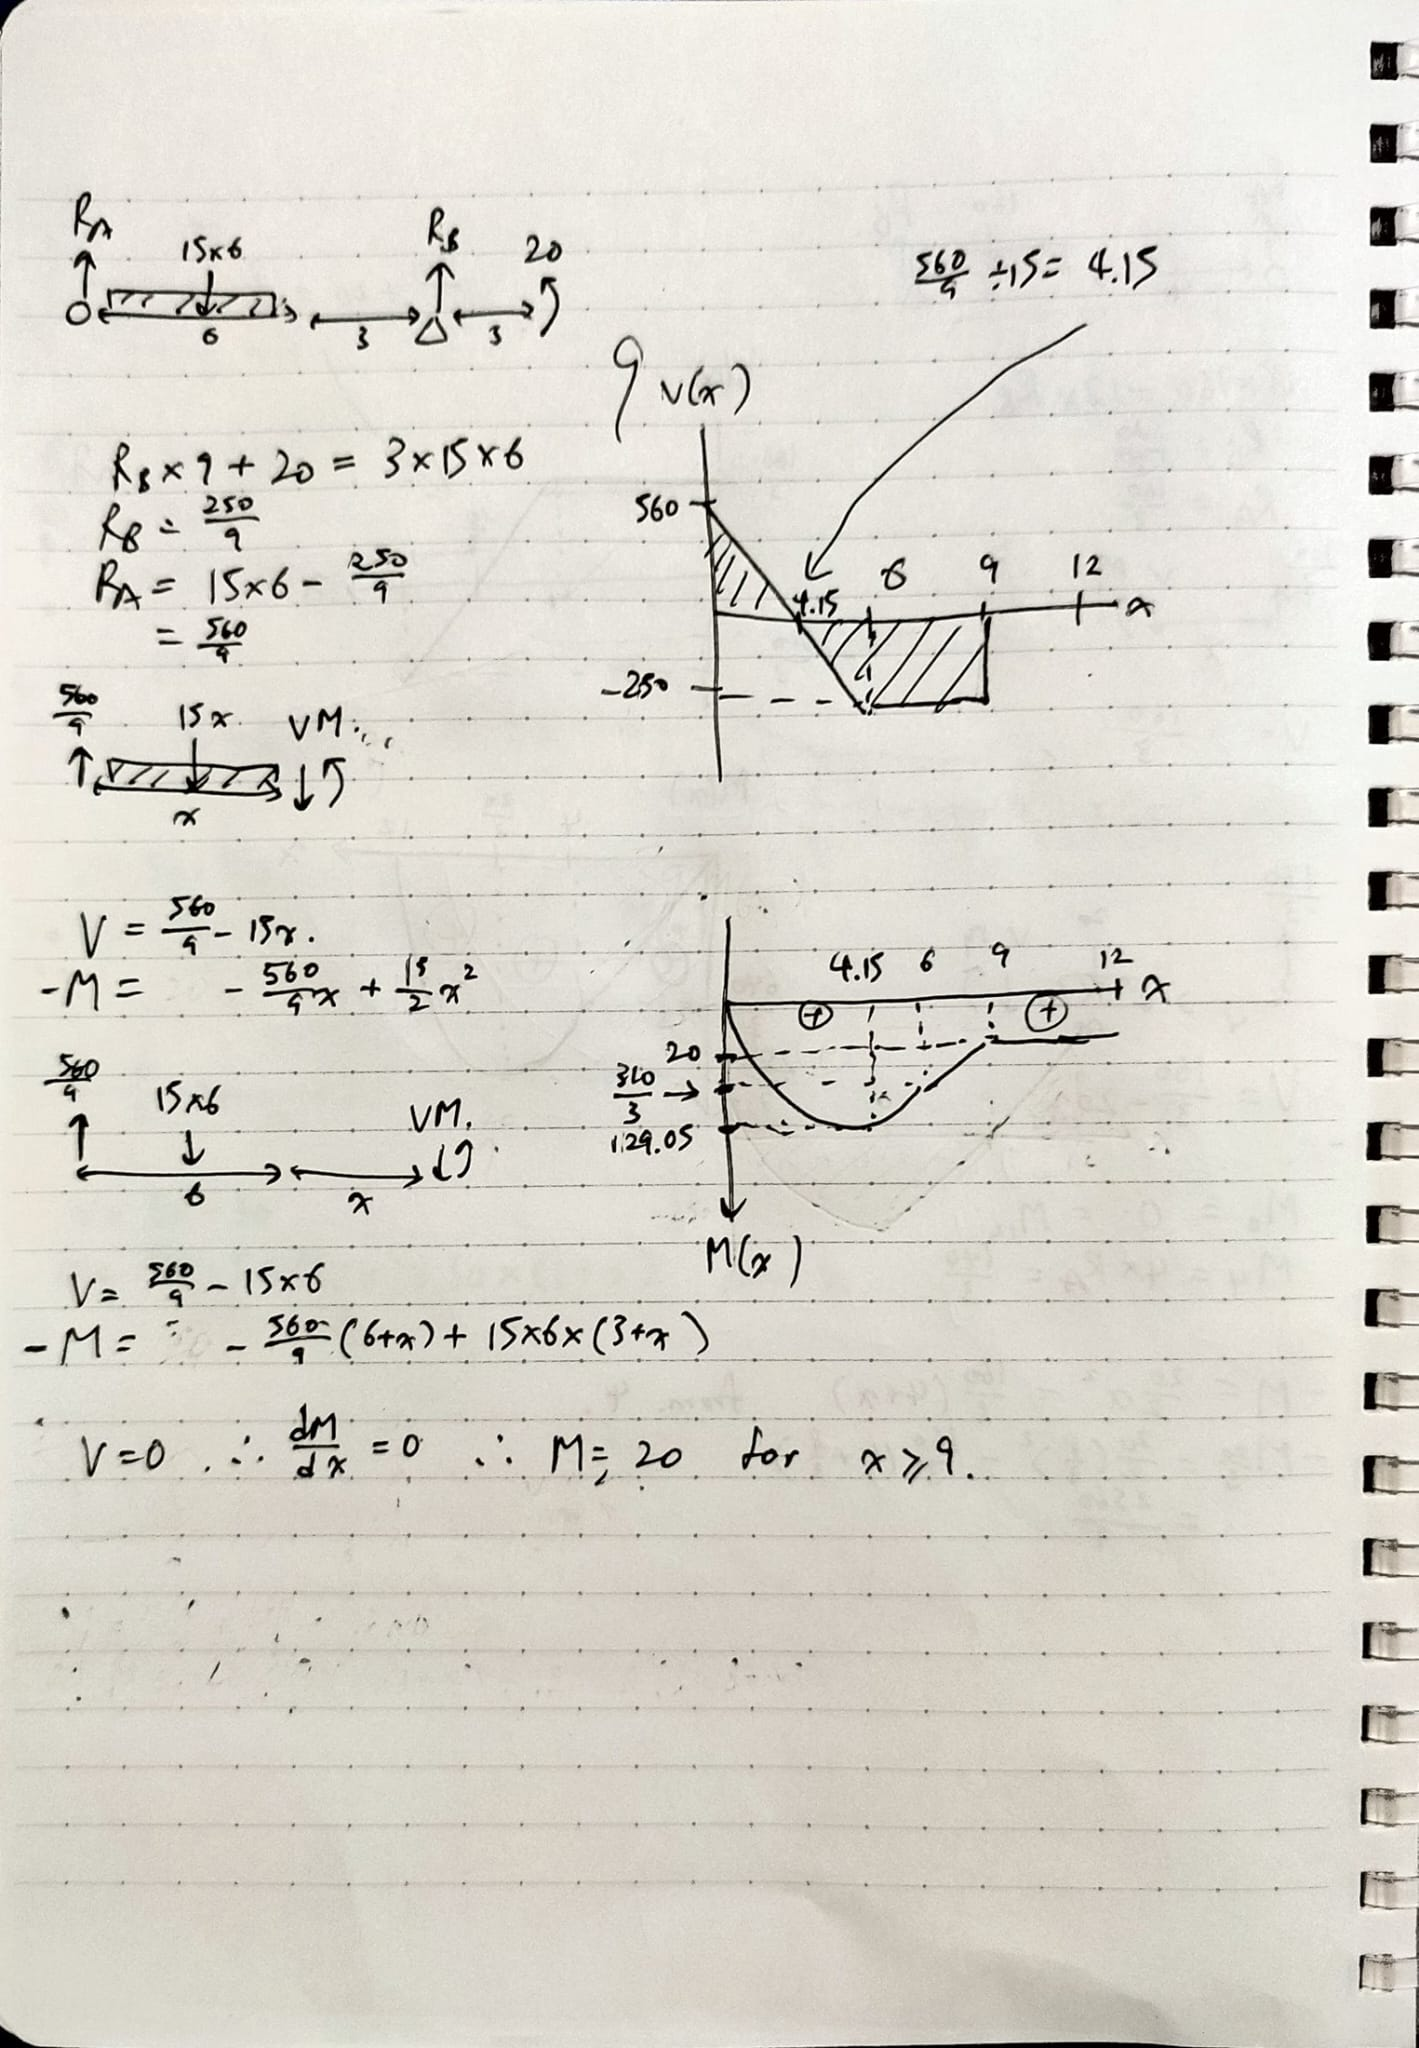
\includegraphics[width=0.7\textwidth]{img/A3Q3.jpeg}

% ------------------------------------ %

\section*{Question 4}
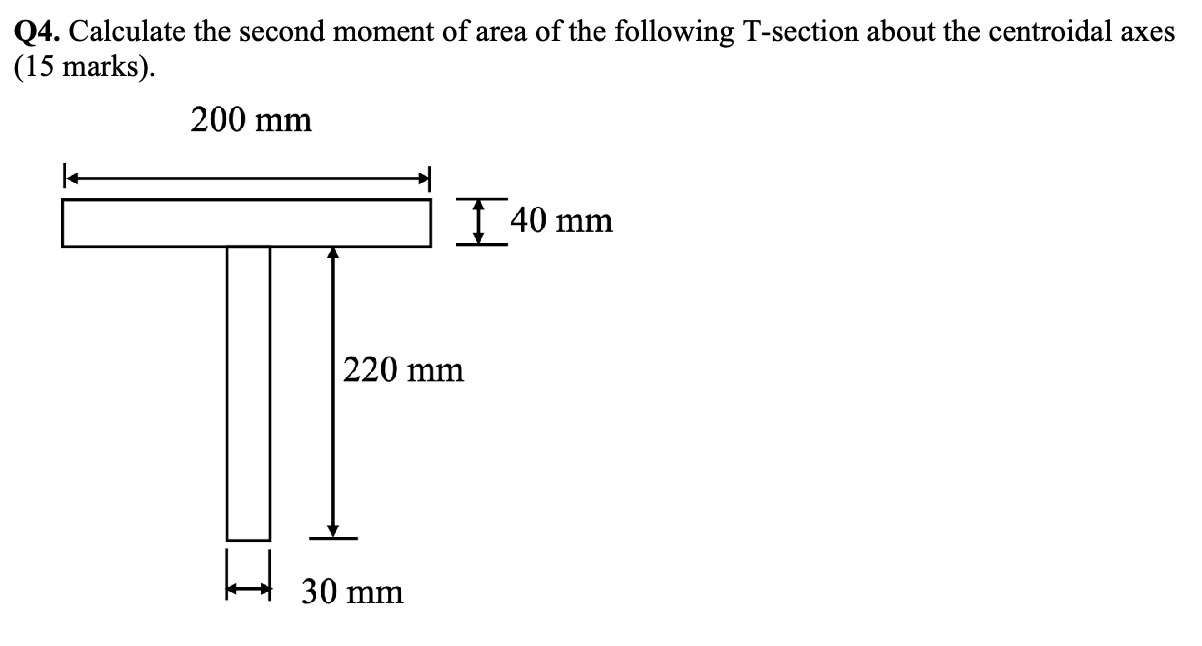
\includegraphics[width=0.6\textwidth]{img/A3Q4.jpg}

Let top rectangle be 1, bottom rectangle be 2. Using centroid distance from top left corner.
\begin{align*}
    \bar{x}   & = 100\ mm                                      \\
    A_1       & = 200 \times 40 = 8000\ mm^2                   \\
    \bar{y_1} & = 20\ mm                                       \\
    A_2       & = 220 \times 30 = 6600\ mm^2                   \\
    \bar{y_2} & = 40 + 110 = 150\ mm                           \\
    \bar{y}   & = \frac{8000\times20+6600\times150}{8000+6600} \\
              & = 78.77\ mm
\end{align*}
\begin{align*}
    I_{xi}=\frac{bh^3}{12} & ,\quad I_{yi}=\frac{hb^3}{12}                                                                     \\
    \\
    I_x                    & = I_{x1\to\bar{y}} + I_{x2\to\bar{y}}                                                             \\
                           & = \frac{b_1h_1^3}{12}+A_1(\bar{y_1}-\bar{y})^2+\frac{b_2h_2^3}{12}+A_2(\bar{y_2}-\bar{y})^2       \\
                           & =\frac{200\times40^3}{12}+8000\times(20-78.77)^2+\frac{30\times220^3}{12}+6600\times(150-78.77)^2 \\
                           & = 88.80\times10^6\ mm^4                                                                           \\
    I_y                    & = I_{y1\to\bar{x}} + I_{y2\to\bar{x}}                                                             \\
                           & = \frac{h_1b_1^3}{12}+\frac{h_2b_2^3}{12}                                                         \\
                           & = \frac{40\times200^3}{12}+\frac{220\times30^3}{12}                                               \\
                           & = 27.16 \times10^6\ mm^4                                                                          \\
\end{align*}

\section*{Question 5}
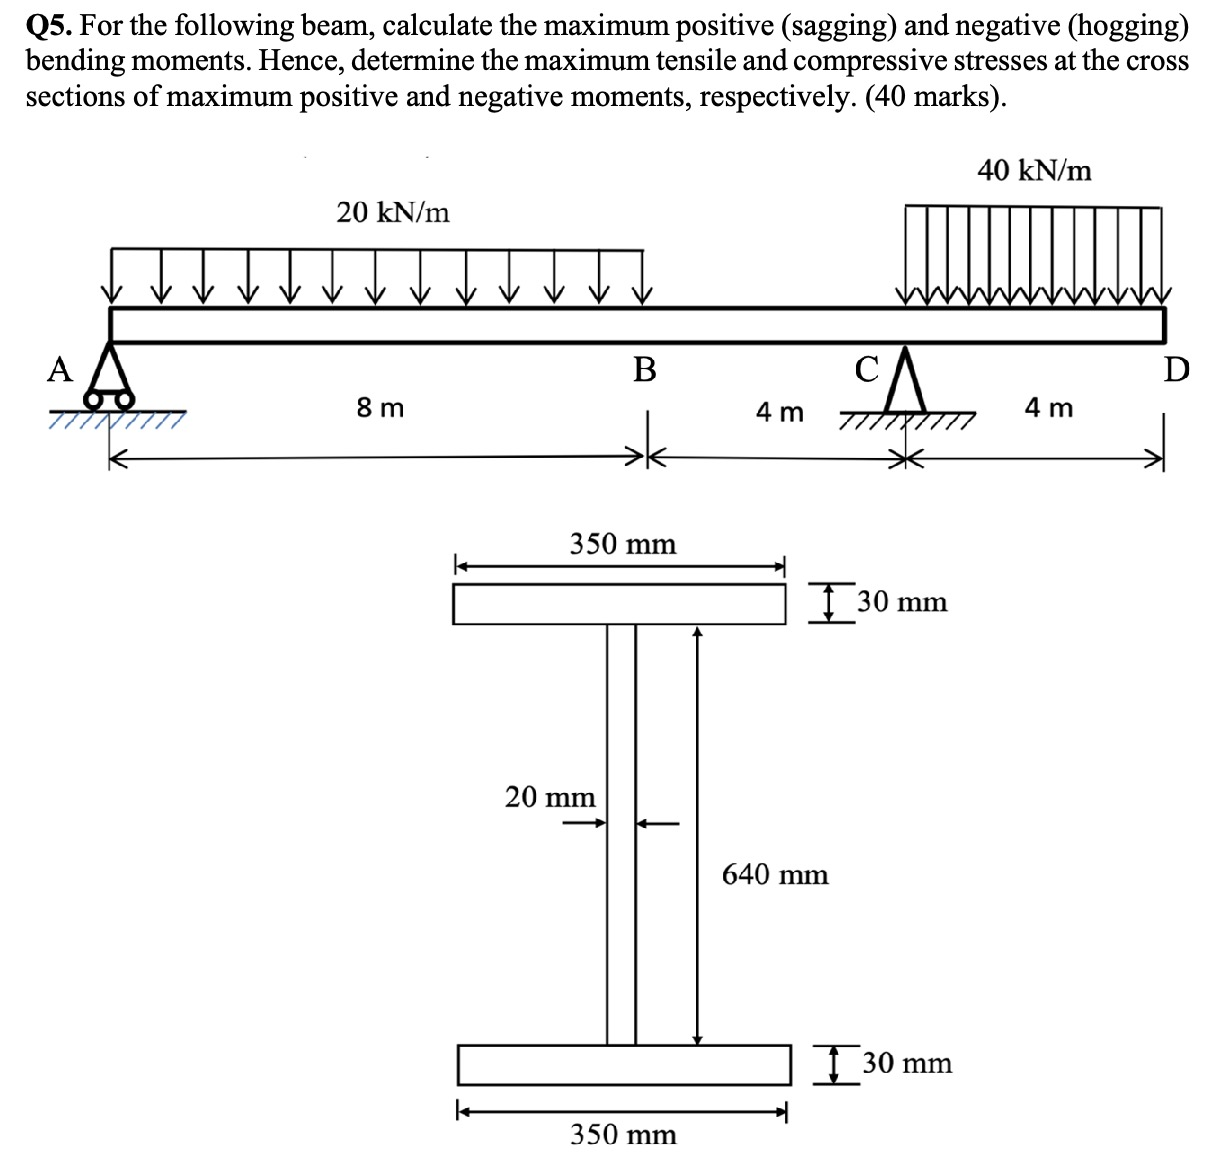
\includegraphics[width=0.6\textwidth]{img/A3Q5.jpg}

Let top rectangle be 1, middle rectangle 2. Using centroid distance from top left corner.
\begin{align*}
    \bar{y} & = 30 + \frac{640}{2} = 350\ mm                                               \\
    A_1     & = 350 \times 30 = 10500\ mm^2 = A_3                                          \\
    A_2     & = 640 \times 20 = 12800\ mm^2                                                \\
    I_x     & = I_{x1\to\bar{y}} + I_{x2\to\bar{y}} + I_{x3\to\bar{y}}                     \\
            & = 2(\frac{350\times30^3}{12}+10500\times(350-15)^2)+\frac{20\times640^3}{12} \\
            & = 2.80\times10^9\ mm^4                                                       \\
            & = 2.80\times10^{-3}\ m^4
\end{align*}
\begin{align*}
    \sum A                                & = 0                                       \\
    20\cdot8\times4+40\cdot4\times(8+4+2) & =R_C\times(8+4)                           \\
    R_C                                   & = 240\ kN                                 \\
    R_A                                   & = 20\cdot8+40\cdot4-240                   \\
                                          & = 80\ kN                                  \\
    -M_{x:0\to8}                          & = 10x^2-80x                               \\
    -M_{>8,\ x:0\to4}                     & = 20\cdot8\times(4+x)-80(8+x)             \\
    -M_{>12,\ x:0\to4}                    & = 20\cdot8\times(8+x)+20x^2-240x-80(12+x) \\
\end{align*}
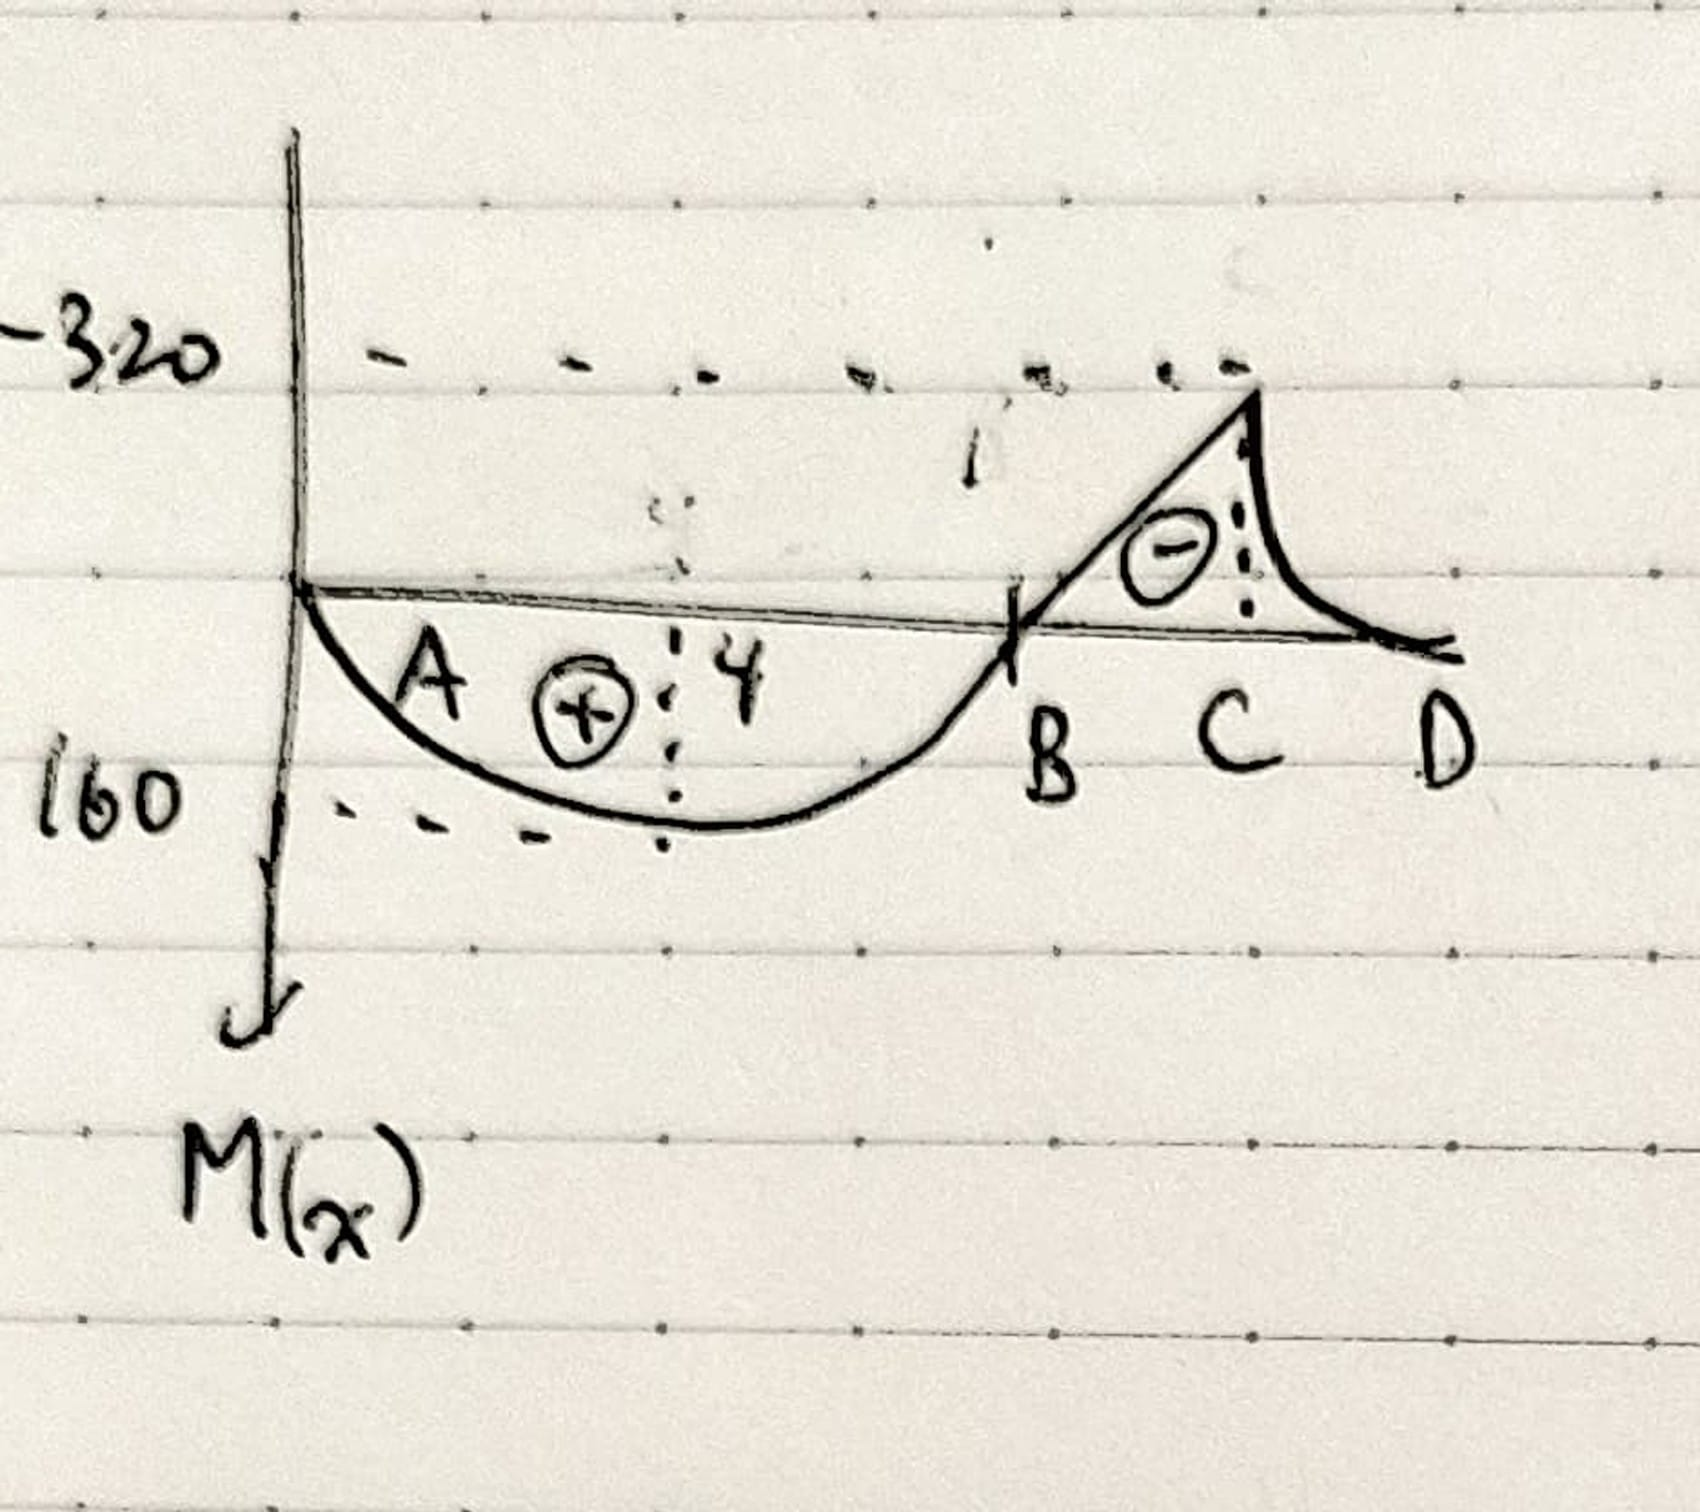
\includegraphics[width=0.5\textwidth]{img/A3Q5-1.jpeg}

Taking tensile stress positive, $y$ downwards positive.
Maximum positive moment and respective values:
\begin{align*}
    M_C            & = -20\cdot8\times(4+4)+80(8+4)             \\
                   & = -320\ Nm\ (\text{hogging})               \\
    \sigma^+_{max} & = \frac{M_D\times y_{max}}{I_x}            \\
                   & = \frac{-320\times 350}{2.80\times10^{-3}} \\
                   & = -40\ MPa                                 \\
    \sigma^-_{max} & = 40\ MPa
\end{align*}
Maximum positive moment and respective values:
\begin{align*}
    M_{4}          & = -10\cdot4^2+80\cdot4                    \\
                   & = 160\ (\text{sagging})                   \\
    \sigma^+_{max} & = \frac{M_{4}\times y_{max}}{I_x}         \\
                   & = \frac{160\times 350}{2.80\times10^{-3}} \\
                   & = 20\ MPa                                 \\
    \sigma^-_{max} & = -20\ MPa
\end{align*}
Note that $\sigma^+$ denotes the bottom of the beam, and $\sigma^-$ denotes the top of the beam.

\end{document}